\chapter{Text classification} \label{Text classification}

Natural language processing (NLP) is the field of designing methods and algorithms that take as input or produce as output unstructured, natural language data \cite{goldberg2017}.
Text classification is a category of tasks in NLP which has many real-world applications such as document classification, spam, bot and fraud detection and web search \cite{howard2018,joulin2016}.
A text classification task requires a training set $D = (d_1, \dots , d_n)$ of labelled documents with class $L \in \mathbb{L}$ (e.g. news, politics, sports). Then the task is to determine a \textit{classification model}
\begin{equation}
  f : D \rightarrow \mathbb{L}\qquad f(d) = L
\end{equation}
which assigns the correct class to in domain document $d$~\cite{hotho}.

The labels are assumed to be purely symbolic so that no additional knowledge of their meaning is available, and the data consists of only knowledge extracted from the documents. Thus metadata such as document type, publication date, etc.\ is not considered available to use.
This ensures that all the methods that will be presented in the coming section are completely general and do not depend on some special-purpose resources.
Given that classification is based on the semantics of documents, which is a subjective notion, the class of a document cannot be deterministically decided.
This lead to the phenomenon called \textit{inter-indexer inconsistency} which manifests itself when two human experts decide if a document $d_j$ should be classified as $c_i$ and disagree on the matter, which happens surprisingly often~\cite{sebastiani2002}.

The automated text classification task dates back to the early '60s but became a major subfield of information systems only in the early '90s due to increased applicative interest and availability of more powerful hardware.
Until the late '80s the most common approach to text classification in real-world applications was a \textit{knowledge engineering} one, which consisted of manually defining a set of rules on how to best classify documents to given categories.
In the '90s this approach was passed in popularity by the \textit{machine learning} paradigm, according to which an automatic text classifier is built by a general inductive process automatically, by learning the characteristics of categories from labelled data \cite{sebastiani2002}.

This chapter gives an overview on text classifiers and other tasks related to training a classifier.
Section \ref{Preprocessing} describes common steps, such as feature extraction and tokenization, that are done before training a classifier, section \ref{Text classifiers} presents various text classification algorithms and models, and finally section \ref{Evaluation} presents metrics for evaluating the performance of a classifier.

\section{Preprocessing}\label{Preprocessing}
Before a machine learning model such as a text classifier can be trained, the data for it has to be preprocessed and mapped to real valued vectors.
Mapping textual data to vectors is called \textit{feature extraction} or \textit{feature representation}.
For a machine learning project it is crucial that the right features for the problem are chosen.
Even though feature engineering is not as important in deep learning, a good set of core features still needs to be defined which is especially true for language data where the data consists of a sequence of discrete symbols.
Somehow this sequence has to be converted into a numerical vector, and in a non-obvious way \cite{goldberg2017}.

\textbf{Tokens} are considered to be the atomic units of NLP.
More often than not, words and tokens are used interchangeably in literature, but a token may consist of multiple words or multiple tokens can represent a single word.
In the next sections, words and tokens are used quite interchangeably.

The following sections describe the features that can be extracted from words and text, and current methods for tokenization.

\subsection{Features of words}\label{Features of words}
The most obvious choice for tokens in NLP are individual words and it is common to do lemmatization or stemming on the words before they are turned into numerical form.

\textbf{Lemmas} are the ``dictionary entries'' of words, for example the lemma of \textit{looking, looked, looks} is \textit{look}.
Determining the lemma of a word is usually done by using lemma lexicons or morphological analyzers.
Adding context into a lemmatizer usually improves the accuracy of lemmatizing given that a lemma can be quite ambiguous without it.
Lemmatization may not work well if words are misspelled or for forms that are not in the lemmatization lexicon.
\textit{Stemming} is a cruder way of determining common forms for words.
It maps sequences of words into shorter sequences so that different inflections map to the same sequence.
The results of stemming do not have to be valid words, e.g.\ picture, pictures and pictured could be stemmed to pictur \cite{goldberg2017}.

\textbf{Distributional information} of words can also be used, e.g.\ what words behave similarly in text.
This distributional information is used in defining vectors for words so that words that behave similarly in text have vectors that are close to each other.
Methods for deriving these vectors are discussed in more detail in chapter \ref{Embeddings}.

\textbf{N-grams} are consecutive word or letter sequences of a given length.
For example, a word-bigram representation of ``the dog is sleeping'' would be [``the dog'', ``dog is'', ``is sleeping''].
Word-bigrams and trigrams - sequences of two and three items - are the most common of the n-grams.
N-grams beyond trigrams are rarely used for words due to sparsity issues although 4-grams and 5-grams are sometimes used for letters \cite{goldberg2017}.

\subsection{Features of text}\label{Features of text}
Sequences of text, such as sentences, can be represented by a number of ways.

\textbf{Bag of words} (BOW) is a common feature extraction procedure used for sentences and documents.
It looks at the histogram of words in a text and considers each word count as a feature.
BOW can be generalized from words to any other word related feature, such as counting word bigrams instead of individual words.

\textbf{Weighting} is used to focus for example on words that appear frequently in a given document, but relatively few times in the whole corpus.
Weighting can be used with the BOW approach, and a common way is to use TF-IDF (Term Frequency - Inverse Document Frequency) weighting which highlights words that are distinctive of the current text.
N-grams can also be used for weighting instead of single words.

\textbf{Windows} focus on the immediate context of a word by considering the $k$ surrounding words, and define features as identities of the words within the window.
It is a version of BOW, but restricted only to the words within the defined window.

\textbf{Position} is an important part of textual data.
A sentence that's words are shuffled will not be equivalent in meaning to the original sentence.
Thus using the positional qualities of words --- such as what the absolute position of a word is in a sentence or does it appear in the first 10 or so words --- as features is also relevant~\cite{goldberg2017}.

\subsection{Tokenization} \label{Tokenization}
The process of tokenization is in charge of splitting text into tokens.
Tokenization is usually done based on white-space and punctuation in languages, such as English, that aren't as morphologically rich.
This approach is called whole-word tokenization as each individual token represents a single word.
In languages such as Hebrew and Arabic, some words attach to the next one without white-space, and in Chinese there is no white-space at all.
Thus, tokenization seems dependent on the language used \cite{goldberg2017}.

In order to circumvent the problems of whole-word tokenization, one can use sub-word tokenization to divide words into multiple tokens.
One such system to extract these tokens is called SentencePiece, which is a widely used tokenizer nowadays.
SentencePiece will be explained in more detail in the next section.


% The following sections describe notable subword tokenization techniques used today.
% \subsubsection{Byte Pair Encoding} \label{Byte Pair Encoding}
% Byte Pair Encoding (BPE)\cite{gage} is a simple data compression technique that iteratively replaces the most frequent pair of bytes in a sequence with a single, unused byte \cite{sennrich2016}.



\subsubsection{SentencePiece} \label{SentencePiece}

SentencePiece is a sub-word tokenizer and detokenizer that is language independent and designed for machine learning -based processing.
It is comprised of four different components: \textbf{Normalizer}, \textbf{Trainer}, \textbf{Encoder} and \textbf{Decoder}.
The Normalizer is used to transform semantically equivalent characters to a canonical form.
The Trainer trains a sub-word segmentation model from the normalized corpus.
The Encoder first normalizes the text with the Normalizer and encodes raw text into a sub-word sequence using the model generated by the Trainer.
The Decoder can be used to transform the tokens into normalized text. \cite{kudo2018}

SentencePiece builds a vocabulary of a predefined size of sub-word tokens.
Depending on the given maximum size, the sub-words' length change.
If, for example, the given maximum size is just 30 or so, the vocabulary could consist of all the letters of the English alphabet and not much else.
On the other hand, if the vocabulary is excessively large, it would essentially work like a whole word tokenizer.
Thus, maximum vocabulary size becomes a tunable hyperparameter for a model, which can have a considerable impact on it's performance.

SentencePiece's language-independent quality is quite important especially for tasks like Neural Machine Translation (NMT), which can perform automatic translation with a simple end-to-end system.
Numerous NMT-systems rely on language dependent pre- and post-processors thus adding sentencepiece to those systems simplifies the processing pipeline and removes the need for custom processors for different languages.

Compared to whole-word tokenization, SentencePiece's sub-word tokenization achieves a lossless representation of data.
For example, a whole word tokenizer might tokenize ``Hello world.'' as [Hello][World][.], thus losing the information of where there is white-space in the sentence.
SentencePiece treats white-space as a normal symbol and replaces all occurrences of white-space with an underscore (U+2581) before tokenization.
SentencePiece might tokenize the aforementioned example as [Hello][\_wor][ld][.], thus preserving the white-space \cite{kudo2018}.

Compared to other sub-word segmentation systems, SentencePiece does not require that the input is pre-tokenized into word sequences.
It works natively with raw sentences which makes a purely language independent and end-to-end system possible \cite{kudo2018}.

SentencePiece seems like a good choice for tokenization for morphologically rich languages such as Finnish.
A version of sub-word tokenization similar to SentencePiece called WordPiece is used in modern models such as BERT (section \ref{BERT}) and ELECTRA (section \ref{ELECTRA}).


\section{Text classifiers} \label{Text classifiers}
\subsection{Naive Bayes} \label{Naive Bayes}
The Naive Bayes Classifier is a probabilistic classifier that assumes that a probabilistic mechanism has generated the words of a document.
It is a simple classifier that estimates the joint probability of a class given a feature vector.
It naively assumes that features are independent given class:
\begin{equation}
  P(X|C) = \prod_{i=1}^{n} P(X_{i}|C)
\end{equation}

Where $X = (X_{1},\cdots, X_{n})$ is a feature vector and $C$ is a class.
Although the assumption is unrealistic, the \textit{Naive Bayes} classifier is surprisingly successful in practice \cite{rish}.

Naive Bayes models are very efficient as they require minimal computational resources even for huge amounts of text and large vocabularies.
However, there exists a significant problem in this approach named the \textit{never-seen-words} problem which manifests itself when a document containing a word that is not present in the training set is analyzed.
The classifier estimates the statistics of a class by counting the occurrences of words in the training set, and a single out-of-vocabulary word will turn the probability of a document belonging to it's according class to 0.
This could turn an otherwise clear-cut classed document into something else only due to a random word \cite{rigutini2004}.

Naive Bayes models have shown good results in various classification tasks and have been used extensively due to their efficiency in training and classification.
A huge setback for the method is its brittleness; to train a robust Naive Bayes Classifier one needs a dataset that covers the problem domain sufficiently, otherwise the model has a high variance.
Thus a small dataset performs significantly worse when using a Naive Bayes Classifier than other document classification methods \cite{rigutini2004} \cite{lewis1998}.

\subsection{Nearest Neighbor Classifier} \label{Nearest Neighbor Classifier}
Nearest neighbor classifiers select documents that are close to the target document instead of building an explicit model.
The class of the document can then be inferred from the classes of the neighbouring documents.
A classifier that selects the k closest documents is called a \textit{k-nearest neighbor classifier} (kNN).
There are a lot of usable measures for similarity such as term frequencies or distributional information.

When deciding if a document belongs to a class, the document has to be compared to all the document in the training set.
Then the k most similar documents are selected and their classes define the probability of whether the document belongs to a certain class or not.
The class that has the largest proportion is then assigned to the document.
Cross-validation can be used to estimate the optimal number for \textit{k} from additional training data \cite{hotho}.

Nearest neighbor classifiers are computationally efficient in practice although they require some computation during classification since to determine the nearest neighbors the distance to all samples has to be calculated \cite{hotho}.
kNNs are more frequently used for unsupervised tasks, such as clustering, rather than supervised tasks \cite{rigutini2004}.



\subsection{Support Vector Machine} \label{Support Vector Machine}
\begin{figure}[t]
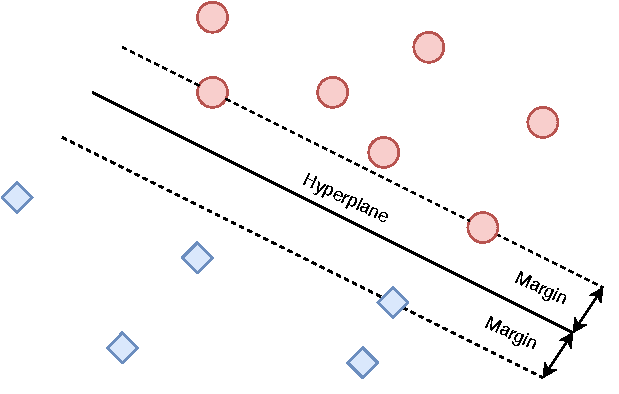
\includegraphics[scale=1.2]{svm}
\centering
\caption{A hyperplane defined by a SVM that separates samples of negative and positive classes with maximal margin}
\label{fig:svm}
\end{figure}

Support vector machines (SVM) are supervised machine learning algorithms that are used for classification and regression analysis.
A single SVM algorithm separates data to two classes by defining a hyperplane that has a maximal distance (margin) to examples of opposing classes (Figure \ref{fig:svm}).
The hyperplane is defined with labeled training data and prediction happens by defining the side in which the example is placed in. If a hyperplane which cuts the data perfectly so that each example is on it's own side is not possible, the algorithm tries to find a division so that as few an example are on the wrong side as possible \cite{hotho}.

In the case that the given classes can not be separated linearly, SVM transforms (``maps'') the input space into a higher dimensional space in which regions can be linearly separated \cite{rigutini2004}.
Support vector machines can also be used for unsupervised learning, when there is no labeled data, to find a natural grouping by using Support Vector Clustering (SVC) \cite{ben-hur2001}.

SVMs have shown good results in text categorization in the past, are quite computationally efficient and generalize well.
Another strength of SVM is that it rarely requires feature selection given that it inherently picks support vectors (individual datapoints) needed for good classification \cite{hotho}.

\subsection{Decision Trees} \label{Decision Trees}

\begin{figure}[t]
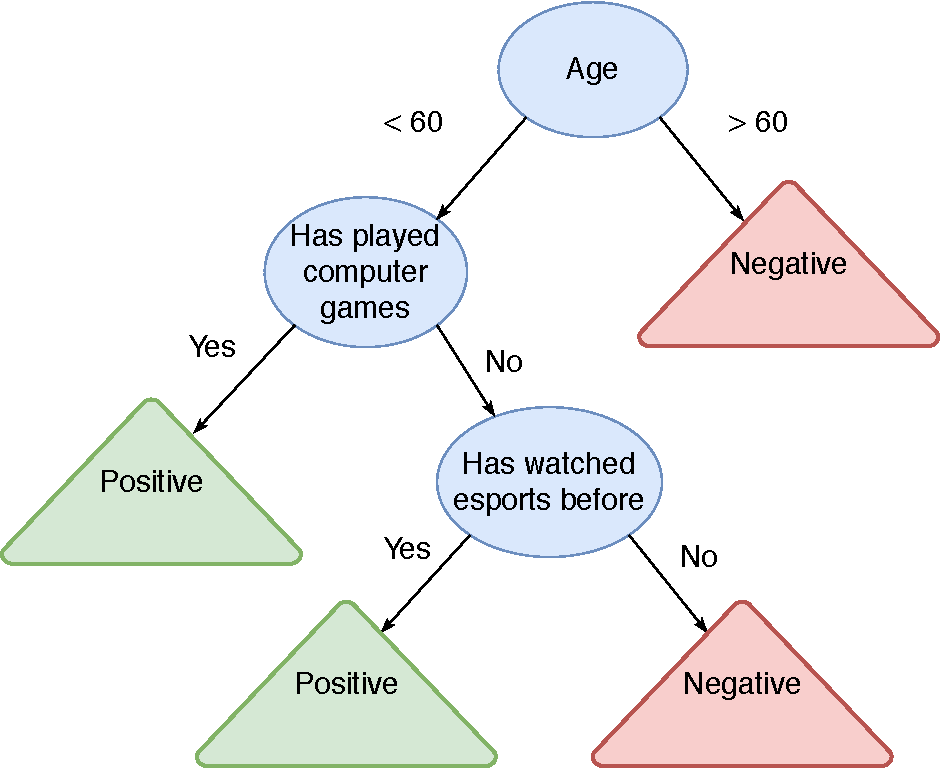
\includegraphics[scale=0.7]{decision_tree}
\centering
\caption{Example of a simple decision tree which predicts the sentiment of a person regarding esports}
\label{fig:decision_tree}
\end{figure}
Decision trees are classifiers that apply a set of rules sequentially to reach a decision.
They can be used for both regression and classification problems and have been among the most popular approaches used for text classification in the past \cite{hotho} \cite{rokach2005}.

Figure \ref{fig:decision_tree} depicts a simple decision tree with three round internal nodes and four triangular leaves.
Nodes are labeled with the testable attribute and branches with the attribute's values.

The training process of a text classification decision tree is as follows: Given a training set $M$ with labelled documents, find the word $t_i$ that best predicts the class of the documents.
Partition the training set into two subsets, $M^+_i$ and $M^-_i$, with $M^+_i$ containing examples with $t_i$ and $M^-_i$ containing examples without $t_i$.
Apply this procedure recursively to $M^+_i$ and $M^-_i$ until all the documents in a subset belong to the same class $L_c$.
The generated tree of rules has an assignment to a class as its leaves \cite{hotho}.

As can be seen from figure \ref{fig:decision_tree}, individual decision trees are quite simple to understand and to interpret, but are usually not competitive with other supervised learning approaches.
They can, however, be dramatically improved by combining multiple trees together to get a consensus prediction with approaches such as \textit{bagging, boosting and random forests} with the cost of losing some interpretability \cite{james2013}.

\subsection{Artificial neural network} \label{Artificial neural network}

A neural network consists of layers of simple processing elements called neurons that are connected to each other.
Each connection has an associated weight that is applied to input.
The first layer is called the input layer after which comes any number of intermediate, or hidden, layers followed by a final output layer.
Neurons are not interconnected within a layer but are only connected to the neurons in adjacent layers.
In a text classifier neural network the prediction of the network can be determined from the values of the final layer's neurons.
For example, a classifier with three different possible classes would have three neurons in the output layer, each corresponding to the probability of a single class \cite{pal1992}.

Neural networks are usually trained using backpropagation which finetunes the parameters --- the weights and biases --- of the network by first feeding the network training data, checking the output and if it is misclassified, and then backtracking and updating the weights of the network to eliminate or minimize the error \cite{sebastiani2002}.

\begin{figure}[t]
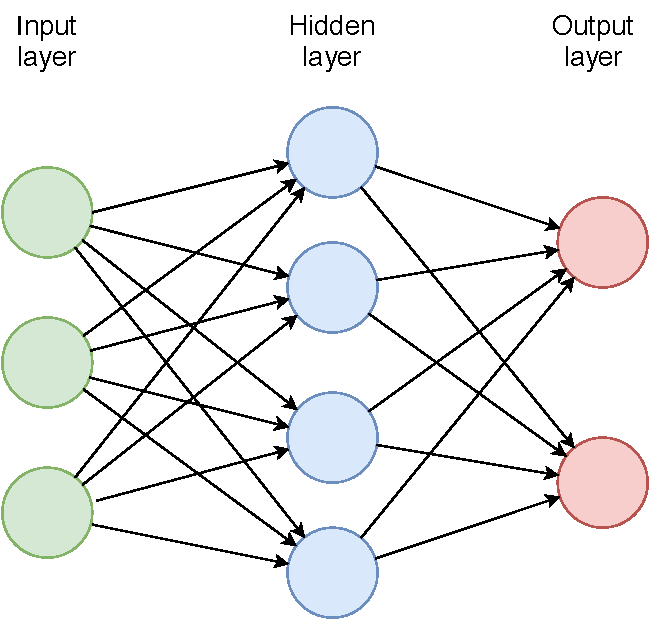
\includegraphics[scale=0.8]{nn}
\centering
\caption{Example of a feedforward neural network}
\label{fig:nn}
\end{figure}

The simplest neural network is the single-layer perceptron, introduced by Rosenblatt in 1958 \cite{rosenblatt1958}, which consists of a single hidden layer between an input layer and an output layer.

Since neural networks consist of simple building blocks, layers of neurons or other functions, stacked on top of each other, it allows designing of deep, complex architectures with practically infinite ways of combination.
The depth of a neural network is defined by the number of it's hidden layers.
The latest state-of-the-art neural network models consist of very deep networks with millions of parameters.

\section{Evaluation} \label{Evaluation}
Evaluating the performance of a classifier is an important step in order to define if the trained classifier actually learned something.

\textbf{True positive, true negative, false positive and false negative} (TP, TN, FP, FN, respectively), are labels used to define the classification result of a single example in a classification task.
If the classifier correctly predicts that the example is positive (e.g. a piece of text belongs to class 1), the example is considered a true positive.
In the case when a negative example is correctly predicted, it is a true negative.
If the classifier wrongly predicts that the example is positive when it is actually negative, or vice versa, the result is a false positive of a false negative.
Depending on the case, a classifier can have requirements such as to minimize the false negative or false positive rate.

Figure \ref{fig:confusionmatrix} depicts a \textbf{confusion matrix} which is a common way to visualize classification results.

\begin{figure}[t]
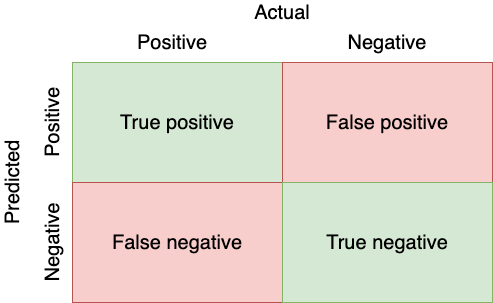
\includegraphics[scale=0.8]{confusionmatrix}
\centering
\caption{A confusion matrix.}
\label{fig:confusionmatrix}
\end{figure}

The simplest metric to use is \textbf{accuracy} (equation \ref{accuracy}), which defines the fraction of correctly classified documents (true positives and true negatives) in relation to the total number of documents.
It is a raw metric that doesn't give a whole lot of insight into the performance of the classifier in such cases where the training data is not evenly distributed.
\begin{equation}\label{accuracy}
  \dfrac{TP + TN}{TP+TN+FP+FN}
\end{equation}

\textbf{Precision} (equation \ref{precision}) defines the accuracy for positive example predictions, e.g. how many of the texts that we classified as 1 were actually 1.
It only takes into account positive predictions that were either true or false.
\begin{equation}\label{precision}
  \dfrac{TP}{TP+FP}
\end{equation}

\textbf{Recall} (equation \ref{recall}) defines the proportion of positive examples actually predicted as positive, e.g. how many of the positive examples did the classifier get right.
\begin{equation}\label{recall}
  \dfrac{TP}{TP+FN}
\end{equation}

\textbf{Specificity} (equation \ref{specificity}) defines the proportion of negative examples that were correctly predicted as negative, e.g. how many of the negative examples did the classifier get right.
Specificity is the opposite of recall.
\begin{equation}\label{specificity}
  \dfrac{TN}{TN+FP}
\end{equation}

\textbf{F-score} or $F_1$ score (equation \ref{fscore}) combines recall and precision in an effort to capture their properties in a single value.
It is the harmonic mean of precision and recall.

\begin{equation}\label{fscore}
  F=\dfrac{2}{1/recall + 1/precision}
\end{equation}

F-score is a commonly used metric to describe system performance in machine learning but it is criticized for lacking detail \cite{derczynski2016}.
Two different models that have the same F-score on the same task are not necessarily successful in the same way.

\textbf{Complementarity} \cite{brill1998} is a measure of the difference in decisions made by two classifiers which attempts to capture the properties that F-score misses.
It represents the amount of times when the other classifier was correct and the other wasn't \cite{derczynski2016}.

Clearly, choosing and reporting only a single metric --- such as accuracy --- as the final performance score of a classifier doesn't truly represent the goodness of a model.
A more full understanding of the shortcomings and strengths of a model is achieved by calculating a number of metrics, such as precision and recall.
